%%%%%%%%%%%%%%%%%%%%%%%%%%%%%%%%%%%%%%%%%%%%%%%%%%%%%%%%%%%%%%%%%%%%%%%%%%%%%%%%
% CHAPTER 1: INTRODUCTION
% Sliding Mode Control for Underactuated Systems
%%%%%%%%%%%%%%%%%%%%%%%%%%%%%%%%%%%%%%%%%%%%%%%%%%%%%%%%%%%%%%%%%%%%%%%%%%%%%%%%

\chapter{Introduction}
\label{ch:introduction}

This chapter introduces the fundamental challenge of controlling underactuated\index{underactuated systems}\index{underactuated systems} mechanical systems and motivates the use of Sliding Mode Control (SMC\index{sliding mode control|see{SMC}}\index{sliding mode control|see{SMC}}) through the benchmark example of the double-inverted pendulum\index{double-inverted pendulum}\index{double-inverted pendulum}. We trace the historical development of SMC from the 1950s to present day, examine the persistent chattering\index{chattering}\index{chattering} problem and modern solutions, and provide an overview of the controllers and software framework developed in this book.

%%%%%%%%%%%%%%%%%%%%%%%%%%%%%%%%%%%%%%%%%%%%%%%%%%%%%%%%%%%%%%%%%%%%%%%%%%%%%%%%
\section{The Challenge of Underactuated Control}
\label{sec:intro:underactuated}

\subsection{Definition and Characteristics}

An underactuated mechanical system is one where the number of independent control inputs is less than the number of degrees of freedom\index{degrees of freedom}\index{degrees of freedom}. Formally, for a system with $n$ degrees of freedom and $m$ independent actuators:

\begin{definition}[Underactuated System]
A mechanical system is \textbf{underactuated} if $m < n$, where:
\begin{itemize}
    \item $n$ = number of degrees of freedom
    \item $m$ = number of independent control inputs
    \item The system cannot instantaneously track arbitrary trajectories in configuration space
\end{itemize}
\end{definition}

\begin{remark}
Underactuation introduces fundamental constraints on controllability\index{controllability}\index{controllability}. Unlike fully actuated systems where every degree of freedom can be directly controlled, underactuated systems require careful exploitation\index{Particle Swarm Optimization!exploitation} of system dynamics (e.g., gravitational potential, centrifugal forces) to achieve desired motions.
\end{remark}

\subsection{Physical Examples}

Underactuated systems appear extensively in robotics, aerospace, and mechanical engineering:

\begin{itemize}
    \item \textbf{Inverted Pendulums}: Cart-pole system (2 DOF, 1 actuator), double-inverted pendulum (3 DOF, 1 actuator)
    \item \textbf{Walking Robots}: Bipedal robots during single-support phase (6+ DOF, 0 actuators at ground contact)
    \item \textbf{Aerial Vehicles}: Quadrotors (6 DOF position/orientation, 4 thrust inputs), helicopters (6 DOF, 4-5 inputs)
    \item \textbf{Marine Vehicles}: Ships and submarines (6 DOF, typically 2-3 propulsion units)
    \item \textbf{Space Robotics}: Free-floating manipulators (12+ DOF, limited actuation)
\end{itemize}

\subsection{Control Challenges}

Underactuated systems present several fundamental challenges:

\begin{enumerate}
    \item \textbf{Limited Controllability}: Not all state variables can be directly commanded
    \item \textbf{Nonlinear Coupling}: Dynamics exhibit strong nonlinear coupling between actuated and unactuated coordinates
    \item \textbf{Sensitivity to Disturbances}: Reduced control authority makes the system more susceptible to external perturbations
    \item \textbf{Complex Stabilization}: Maintaining equilibrium\index{equilibrium}\index{equilibrium} requires continuous feedback\index{feedback control} (unlike fully actuated systems where static feedback may suffice)
    \item \textbf{Nonholonomic Constraints}: Some underactuated systems have velocity-dependent constraints that further limit reachable configurations
\end{enumerate}

\begin{example}[Cart-Pole Controllability]
Consider the cart-pole\index{cart-pole system}\index{cart-pole system} system with state $x = [x_{\text{cart}}, \theta, \dot{x}_{\text{cart}}, \dot{\theta}]^T$. The control input\index{control input}\index{control input} $u$ (cart force) can directly affect $\ddot{x}_{\text{cart}}$, but $\ddot{\theta}$ is only indirectly influenced through the nonlinear coupling term:
\begin{equation}
\ddot{\theta} = f(x, \dot{x}, u) \propto u \cos\theta + \text{nonlinear terms}
\end{equation}
At $\theta = \pi/2$ (horizontal pendulum), the coupling term vanishes ($\cos(\pi/2) = 0$), creating a singularity in controllability.
\end{example}

%%%%%%%%%%%%%%%%%%%%%%%%%%%%%%%%%%%%%%%%%%%%%%%%%%%%%%%%%%%%%%%%%%%%%%%%%%%%%%%%
\section{The Double-Inverted Pendulum as a Benchmark System}
\label{sec:intro:dip}

\subsection{System Description}

The double-inverted pendulum (DIP\index{double-inverted pendulum|see{DIP}}\index{double-inverted pendulum|see{DIP}}) consists of two rigid links connected in series, mounted on a cart that moves horizontally along a rail. This system serves as an ideal benchmark for underactuated control research due to its:

\begin{itemize}
    \item \textbf{High Nonlinearity}: Trigonometric terms in equations of motion
    \item \textbf{Significant Coupling}: Motion of the cart affects both pendula, and pendulum motion affects each other
    \item \textbf{Unstable Equilibrium}: The upright position is naturally unstable
    \item \textbf{Measurable Complexity}: 3 degrees of freedom, 6-dimensional state space\index{state space}\index{state space}, 1 control input
    \item \textbf{Computational Tractability}: Simulation and control implementation are feasible on standard hardware
\end{itemize}

\begin{figure}[htbp]
\centering
% Double Inverted Pendulum Schematic
% TikZ diagram for Chapter 1

\begin{tikzpicture}[scale=1.2]
    % Ground
    \fill[pattern=north east lines] (-2, -0.3) rectangle (2, 0);
    \draw[thick] (-2, 0) -- (2, 0);

    % Cart
    \draw[thick, fill=gray!20] (-0.6, 0) rectangle (0.6, 0.8);
    \node at (0, 0.4) {\textbf{Cart}};
    \node[below] at (0, -0.15) {$M$};

    % Wheels
    \draw[fill=black] (-0.4, 0) circle (0.15);
    \draw[fill=black] (0.4, 0) circle (0.15);

    % Force arrow
    \draw[->, ultra thick, red] (0.8, 0.4) -- (1.6, 0.4) node[midway, above] {$u(t)$};

    % First pendulum (link 1)
    \coordinate (pivot1) at (0, 0.8);
    \coordinate (mass1) at ({0.8*sin(25)}, {0.8 + 0.8*cos(25)});

    \draw[thick, blue] (pivot1) -- (mass1);
    \draw[fill=blue!30] (mass1) circle (0.2);
    \node at (mass1) {$m_1$};

    % Angle arc for theta1
    \draw[->] (0, 1.2) arc (90:65:0.4);
    \node at (0.3, 1.35) {$\theta_1$};

    % Length label L1
    \draw[<->, dashed] (0.15, 0.8) -- (0.15, {0.8 + 0.4*cos(25)});
    \node[right] at (0.15, {0.8 + 0.2}) {$L_1$};

    % Second pendulum (link 2)
    \coordinate (pivot2) at (mass1);
    \coordinate (mass2) at ({0.8*sin(25) + 0.6*sin(35)}, {0.8 + 0.8*cos(25) + 0.6*cos(35)});

    \draw[thick, green!50!black] (pivot2) -- (mass2);
    \draw[fill=green!30] (mass2) circle (0.18);
    \node at (mass2) {$m_2$};

    % Angle arc for theta2
    \draw[->] (mass1) ++({0.3*sin(25)}, {0.3*cos(25)}) arc (90:55:0.3);
    \node at ({0.8*sin(25) + 0.25}, {0.8 + 0.8*cos(25) + 0.25}) {$\theta_2$};

    % Length label L2
    \draw[<->, dashed] ({0.8*sin(25) + 0.1}, {0.8 + 0.8*cos(25)}) --
                       ({0.8*sin(25) + 0.1}, {0.8 + 0.8*cos(25) + 0.3*cos(35)});
    \node[right] at ({0.8*sin(25) + 0.1}, {0.8 + 0.8*cos(25) + 0.15}) {$L_2$};

    % Cart position x
    \draw[<->, thick] (-1.5, -0.6) -- (0, -0.6);
    \node[below] at (-0.75, -0.6) {$x(t)$};

    % Coordinate system
    \draw[->, thick] (2.5, -0.5) -- (3.2, -0.5) node[right] {$x$};
    \draw[->, thick] (2.5, -0.5) -- (2.5, 0.2) node[above] {$y$};

    % Reference dashed lines (vertical)
    \draw[dashed, gray] (0, 0.8) -- (0, 2.5);
    \draw[dashed, gray] (mass1) -- ({0.8*sin(25)}, 2.5);

\end{tikzpicture}

\caption[Double-Inverted Pendulum System Overview]{System overview of the double-inverted pendulum benchmark. The cart (mass $M$) moves horizontally along a rail under control force $u$. Two pendula (masses $m_1, m_2$, lengths $L_1, L_2$) are connected in series. Angles $\theta_1$ and $\theta_2$ are measured from the vertical, with the upright equilibrium at $\theta_1 = \theta_2 = 0$. This system has 3 DOF ($x_{\text{cart}}, \theta_1, \theta_2$) but only 1 actuator ($u$), making it underactuated with 67\% underactuation ratio.}
\label{fig:intro:dip_schematic}
\end{figure}

\subsection{Equations of Motion}

The dynamics of the DIP are derived using Lagrangian\index{Lagrangian mechanics}\index{Lagrangian mechanics} mechanics (detailed derivation in \cref{ch:mathematical_foundations}). The equations of motion have the form:

\begin{equation}
\label{eq:intro:dip_dynamics}
\mat{M}(\vect{q}) \ddot{\vect{q}} + \mat{C}(\vect{q}, \dot{\vect{q}}) \dot{\vect{q}} + \vect{G}(\vect{q}) + \vect{F}(\dot{\vect{q}}) = \mat{B} u
\end{equation}

where:
\begin{itemize}
    \item $\vect{q} = [x_{\text{cart}}, \theta_1, \theta_2]^T \in \Real^3$ is the generalized coordinate vector
    \item $\mat{M}(\vect{q}) \in \Real^{3 \times 3}$ is the configuration-dependent inertia matrix\index{inertia matrix}\index{inertia matrix}
    \item $\mat{C}(\vect{q}, \dot{\vect{q}}) \in \Real^{3 \times 3}$ captures Coriolis\index{Coriolis forces}\index{Coriolis forces} and centrifugal forces
    \item $\vect{G}(\vect{q}) \in \Real^3$ is the gravitational force\index{gravitational force}\index{gravitational force} vector
    \item $\vect{F}(\dot{\vect{q}}) \in \Real^3$ represents viscous friction
    \item $\mat{B} = [1, 0, 0]^T$ is the input distribution matrix (force acts only on cart)
    \item $u \in \Real$ is the control force
\end{itemize}

\begin{remark}
The inertia matrix $\mat{M}(\vect{q})$ is symmetric and positive definite for all configurations, ensuring physical realizability. However, its entries depend nonlinearly on $\theta_1$ and $\theta_2$ (through $\cos(\theta_2 - \theta_1)$ terms), complicating controller design.
\end{remark}

\subsection{Why the DIP is an Ideal Benchmark}

The double-inverted pendulum has become a standard benchmark in nonlinear control research for several reasons:

\begin{enumerate}
    \item \textbf{Challenging Dynamics}: The system exhibits fast unstable modes, nonlinear coupling, and sensitivity to initial conditions
    \item \textbf{Well-Defined Control Objectives}: Stabilization around upright equilibrium ($\theta_1 = \theta_2 = 0$) provides a clear success criterion
    \item \textbf{Hardware Realizability}: Physical prototypes can be built at reasonable cost, enabling experimental validation
    \item \textbf{Scalability}: Concepts developed for DIP generalize to higher-dimensional underactuated systems (e.g., triple pendulum, Acrobot)
    \item \textbf{Rich Behavior}: The system supports multiple control tasks (stabilization\index{stabilization}, swing-up\index{swing-up control}, trajectory tracking\index{trajectory tracking}), enabling comprehensive algorithm testing
\end{enumerate}

\begin{figure}[htbp]
\centering
% Control Objectives Illustration
% TikZ diagram for Chapter 1

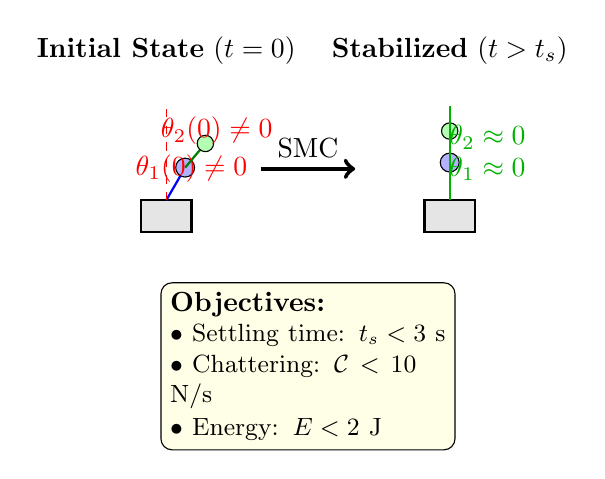
\begin{tikzpicture}[scale=0.8]
    % Initial state
    \begin{scope}
        \node[above] at (0, 2.5) {\textbf{Initial State} ($t=0$)};

        % Cart
        \draw[thick, fill=gray!20] (-0.4, 0) rectangle (0.4, 0.5);

        % Pendula (perturbed)
        \draw[thick, blue] (0, 0.5) -- ({0.6*sin(30)}, {0.5 + 0.6*cos(30)});
        \draw[fill=blue!30] ({0.6*sin(30)}, {0.5 + 0.6*cos(30)}) circle (0.15);

        \draw[thick, green!50!black] ({0.6*sin(30)}, {0.5 + 0.6*cos(30)}) --
                                     ({0.6*sin(30) + 0.5*sin(40)}, {0.5 + 0.6*cos(30) + 0.5*cos(40)});
        \draw[fill=green!30] ({0.6*sin(30) + 0.5*sin(40)}, {0.5 + 0.6*cos(30) + 0.5*cos(40)}) circle (0.13);

        % Reference vertical
        \draw[dashed, red] (0, 0.5) -- (0, 2);

        % Angles
        \node[red] at (0.4, 1.0) {$\theta_1(0) \neq 0$};
        \node[red] at (0.8, 1.6) {$\theta_2(0) \neq 0$};
    \end{scope}

    % Arrow
    \draw[->, ultra thick] (1.5, 1) -- (3, 1) node[midway, above] {SMC};

    % Final state (stabilized)
    \begin{scope}[xshift=4.5cm]
        \node[above] at (0, 2.5) {\textbf{Stabilized} ($t > t_s$)};

        % Cart
        \draw[thick, fill=gray!20] (-0.4, 0) rectangle (0.4, 0.5);

        % Pendula (upright)
        \draw[thick, blue] (0, 0.5) -- (0, 1.1);
        \draw[fill=blue!30] (0, 1.1) circle (0.15);

        \draw[thick, green!50!black] (0, 1.1) -- (0, 1.6);
        \draw[fill=green!30] (0, 1.6) circle (0.13);

        % Reference vertical (overlapping)
        \draw[thick, green!70!black] (0, 0.5) -- (0, 2);

        % Check marks
        \node[green!70!black] at (0.6, 1.0) {$\theta_1 \approx 0$ \checkmark};
        \node[green!70!black] at (0.6, 1.5) {$\theta_2 \approx 0$ \checkmark};
    \end{scope}

    % Performance metrics
    \node[below, align=left, draw, rounded corners, fill=yellow!10, text width=3.5cm] at (2.25, -0.8) {
        \textbf{Objectives:}\\
        \small
        $\bullet$ Settling time: $t_s < 3$ s\\
        $\bullet$ Chattering: $\mathcal{C} < 10$ N/s\\
        $\bullet$ Energy: $E < 2$ J
    };

\end{tikzpicture}

\caption[Control Objectives for DIP Stabilization]{Illustration of control objectives for double-inverted pendulum stabilization. \textbf{Left:} Initial perturbed state with $\theta_1(0) \neq 0$, $\theta_2(0) \neq 0$ deviating from vertical reference (dashed red line). \textbf{Right:} Final stabilized state achieved through SMC, with both pendula upright ($\theta_1 \approx 0$, $\theta_2 \approx 0$) within settling time $t_s < 3$ s. Performance metrics include settling time, chattering suppression ($\mathcal{C} < 10$ N/s), and energy consumption ($E < 2$ J).}
\label{fig:intro:control_objectives}
\end{figure}

%%%%%%%%%%%%%%%%%%%%%%%%%%%%%%%%%%%%%%%%%%%%%%%%%%%%%%%%%%%%%%%%%%%%%%%%%%%%%%%%
\section{Historical Development of Sliding Mode Control (1950s--2025)}
\label{sec:intro:smc_history}

\subsection{Origins: Variable Structure Systems (1950s--1960s)}

Sliding mode control originated in the Soviet Union during the 1950s as part of the broader study of \textit{variable structure systems} (VSS). Pioneering work by Emelyanov and colleagues~\cite{emelyanov1967variable} established the fundamental concept: a control law that switches between multiple feedback structures based on the system state.

\begin{definition}[Variable Structure System]
A control system is a \textbf{variable structure system} if its feedback law switches discontinuously among multiple predefined control structures:
\begin{equation}
u(x) = \begin{cases}
u^{(1)}(x), & \text{if } \sigma(x) > 0 \\
u^{(2)}(x), & \text{if } \sigma(x) < 0
\end{cases}
\end{equation}
where $\sigma(x) : \Real^n \to \Real$ is the \textbf{switching function}.
\end{definition}

The key insight was that by designing the switching function appropriately, the system trajectory could be forced onto a manifold (the \textit{sliding surface}) where desirable dynamics emerge.

\subsection{Theoretical Foundations (1970s--1980s)}

The 1970s and 1980s saw the development of rigorous mathematical foundations for SMC:

\begin{itemize}
    \item \textbf{Utkin's Seminal Work (1977)}: Vadim Utkin formalized SMC theory~\cite{utkin1977variable}, establishing:
    \begin{itemize}
        \item The \textit{reaching condition} ($\sigma \dot{\sigma} < 0$) ensures finite-time convergence\index{convergence} to the sliding surface
        \item The \textit{equivalent control method} for analyzing sliding mode dynamics
        \item Robustness to \textit{matched disturbances} (perturbations entering through the control channel)
    \end{itemize}

    \item \textbf{Filippov Solutions (1960s-1980s)}: Filippov's theory of differential equations with discontinuous right-hand sides~\cite{filippov1988differential} provided the mathematical framework for analyzing SMC systems where $u(x)$ is discontinuous.

    \item \textbf{Lyapunov-Based Design (1980s)}: Development of Lyapunov function methods to systematically prove stability\index{stability}\index{stability} and convergence of SMC laws.
\end{itemize}

\subsection{Chattering Problem and Boundary Layer Method (1980s)}

A major limitation of classical SMC\index{sliding mode control!classical}\index{sliding mode control!classical} emerged: \textit{chattering}---high-frequency oscillations around the sliding surface caused by imperfect control switching. Burton and Zinober~\cite{burton1986continuous} proposed the \textit{boundary layer method}:

\begin{equation}
\text{sign}(\sigma) \to \sat(\sigma/\epsilon) = \begin{cases}
\sigma/\epsilon, & \text{if } |\sigma| \leq \epsilon \\
\text{sign}(\sigma), & \text{if } |\sigma| > \epsilon
\end{cases}
\end{equation}

This continuous approximation eliminates chattering at the cost of a small steady-state tracking error\index{performance metrics!tracking error} bounded by the boundary layer thickness $\epsilon$.

\subsection{Higher-Order Sliding Modes (1990s--2000s)}

To eliminate chattering without sacrificing tracking accuracy, Levant developed \textit{higher-order sliding modes}~\cite{levant2003higher}:

\begin{itemize}
    \item \textbf{Second-Order SMC}: The discontinuity is applied to the control \textit{derivative} ($\dot{u}$) rather than the control itself, resulting in continuous control signals
    \item \textbf{Super-Twisting Algorithm (STA)}: A specific second-order SMC law:
    \begin{align}
    u &= -K_1 \sqrt{|\sigma|} \sign(\sigma) + u_{\text{int}} \\
    \dot{u}_{\text{int}} &= -K_2 \sign(\sigma)
    \end{align}
    Achieves \textit{finite-time convergence} of both $\sigma$ and $\dot{\sigma}$ to zero, eliminating chattering while maintaining robustness\index{robustness}\index{robustness}.
\end{itemize}

\subsection{Adaptive and Intelligent SMC (2000s--2010s)}

The 2000s saw integration of SMC with adaptive control and computational intelligence:

\begin{itemize}
    \item \textbf{Adaptive Gain Tuning}: Online adjustment of switching gains based on observed disturbances, eliminating the need for conservative a priori bounds~\cite{yang2007adaptive}
    \item \textbf{Neural Network SMC}: Approximation of unknown dynamics using neural networks~\cite{huang2008adaptive}
    \item \textbf{Fuzzy SMC}: Fuzzy logic for gain scheduling and chattering reduction
    \item \textbf{Optimization-Based Tuning}: Particle Swarm Optimization\index{Particle Swarm Optimization}\index{Particle Swarm Optimization} (PSO\index{Particle Swarm Optimization|see{PSO}}\index{Particle Swarm Optimization|see{PSO}}) and genetic algorithms for systematic gain selection~\cite{messina2013multiobjective}
\end{itemize}

\subsection{Recent Advances (2010s--Present)}

Contemporary SMC research focuses on:

\begin{itemize}
    \item \textbf{Prescribed-Time Convergence}: SMC laws that guarantee convergence within a user-specified time, independent of initial conditions
    \item \textbf{Barrier Functions}: Integrating control barrier functions with SMC to enforce state constraints
    \item \textbf{Event-Triggered SMC}: Reducing control update frequency by switching only when a Lyapunov-based criterion is violated
    \item \textbf{Data-Driven SMC}: Learning sliding surface designs directly from data without explicit system models
    \item \textbf{Fractional-Order SMC}: Extending SMC to fractional-order systems with non-integer differential operators
\end{itemize}

%%%%%%%%%%%%%%%%%%%%%%%%%%%%%%%%%%%%%%%%%%%%%%%%%%%%%%%%%%%%%%%%%%%%%%%%%%%%%%%%
\section{The Chattering Problem and Modern Solutions}
\label{sec:intro:chattering}

\subsection{Physical Manifestation}

Chattering is the most significant practical limitation of classical SMC. It manifests as:

\begin{itemize}
    \item \textbf{High-Frequency Control Oscillations}: Control signal $u(t)$ switches rapidly (100--1000 Hz) around the sliding surface
    \item \textbf{Actuator Wear}: Mechanical actuators (motors, valves) subjected to rapid switching experience accelerated wear
    \item \textbf{Excitation of Unmodeled Dynamics}: High-frequency content excites flexible modes, sensor dynamics, and other unmodeled phenomena
    \item \textbf{Acoustic Noise}: Audible chattering in mechanical systems
\end{itemize}

\subsection{Root Causes}

Chattering arises from several sources:

\begin{enumerate}
    \item \textbf{Discrete-Time Implementation}: Digital controllers sample at finite frequency, converting the ideal sliding mode into a \textit{quasi-sliding mode} with zigzag motion around the surface
    \item \textbf{Switching Delays}: Actuators have nonzero response time, preventing instantaneous switching
    \item \textbf{Measurement Noise}: Sensor noise\index{sensor noise} causes spurious crossings of the sliding surface
    \item \textbf{Unmodeled Dynamics}: High-frequency modes interact with the discontinuous control, creating limit cycles
\end{enumerate}

\begin{figure}[htbp]
\centering
\includegraphics[width=0.8\textwidth]{figures/placeholder_chattering_illustration.png}
\caption[Chattering Phenomenon in SMC]{Illustration of chattering in sliding mode control. The ideal sliding mode (smooth convergence to $\sigma = 0$) is shown in blue. The practical implementation exhibits rapid oscillations (chattering) around the sliding surface due to sampling delays, actuator dynamics, and measurement noise. The boundary layer method (green) eliminates chattering at the cost of steady-state error bounded by $\epsilon$.}
\label{fig:intro:chattering}
\end{figure}

\subsection{Mitigation Strategies}

Several approaches have been developed to reduce or eliminate chattering:

\begin{table}[htbp]
\centering
\caption[Comparison of Chattering Reduction Methods]{Comparison of Five Chattering Reduction Methods in Sliding Mode Control: Boundary layer smoothing, higher-order SMC (Super-Twisting\index{Super-Twisting Algorithm|see{STA}} Algorithm), observer-based filtering, adaptive gain scheduling, and disturbance observer compensation. Each method involves distinct trade-offs between chattering\index{chattering} suppression, steady-state accuracy, computational complexity, and robustness\index{robustness}.}
\label{tab:intro:chattering_methods}
\begin{tabular}{lp{6cm}p{4cm}}
\toprule
\textbf{Method} & \textbf{Description} & \textbf{Trade-off} \\
\midrule
Boundary Layer & Replace $\sign(\sigma)$ with $\sat(\sigma/\epsilon)$ & Steady-state error $\sim \epsilon$ \\
\midrule
Higher-Order SMC & Apply discontinuity to $\dot{u}$ instead of $u$ & Increased computational complexity \\
\midrule
Observer-Based & Use state observer to filter measurements & Observer design complexity \\
\midrule
Adaptive Gains & Adjust switching gain based on $|\sigma|$ & Requires careful adaptation law tuning \\
\midrule
Disturbance Observer & Estimate and compensate disturbances explicitly & Sensitive to model accuracy \\
\bottomrule
\end{tabular}
\end{table}

%%%%%%%%%%%%%%%%%%%%%%%%%%%%%%%%%%%%%%%%%%%%%%%%%%%%%%%%%%%%%%%%%%%%%%%%%%%%%%%%
\section{Overview of Controllers Covered in This Book}
\label{sec:intro:controllers}

This book presents a comprehensive suite of SMC controllers for underactuated systems, ranging from classical first-order SMC to advanced hybrid adaptive\index{sliding mode control!hybrid adaptive}\index{sliding mode control!hybrid adaptive} algorithms. Each controller is derived rigorously, implemented in production-quality Python\index{Python implementation}\index{Python implementation} code, and validated experimentally on the DIP benchmark.

\subsection{Classical Sliding Mode Control (Chapter \ref{ch:classical_smc})}

\textbf{Key Features}:
\begin{itemize}
    \item First-order sliding mode with linear sliding surface
    \item Boundary layer for chattering reduction (tanh or linear saturation)
    \item Equivalent control based on DIP dynamics
    \item Exponential convergence to sliding surface
\end{itemize}

\textbf{Control Law}:
\begin{equation}
u = u_{\text{eq}} - K \sat(\sigma/\epsilon) - k_d \sigma
\end{equation}

\subsection{Super-Twisting Algorithm (Chapter \ref{ch:super_twisting})}

\textbf{Key Features}:
\begin{itemize}
    \item Second-order sliding mode (continuous control signal)
    \item Finite-time convergence of $\sigma$ and $\dot{\sigma}$ to zero
    \item Chattering elimination without boundary layer trade-off
    \item Robust to Lipschitz-continuous disturbances
\end{itemize}

\textbf{Control Law}:
\begin{align}
u &= -K_1 \sqrt{|\sigma|} \sat(\sigma/\epsilon) + u_{\text{int}} + u_{\text{eq}} \\
\dot{u}_{\text{int}} &= -K_2 \sat(\sigma/\epsilon)
\end{align}

\subsection{Adaptive Sliding Mode Control (Chapter 5)}

\textbf{Key Features}:
\begin{itemize}
    \item Online adaptation of switching gain $K(t)$
    \item No a priori knowledge of disturbance bounds required
    \item Dead zone to prevent noise-induced gain windup
    \item Leak term to handle time-varying disturbances
\end{itemize}

\textbf{Adaptation Law}:
\begin{equation}
\dot{K}(t) = \begin{cases}
\gamma |\sigma|, & \text{if } |\sigma| > \delta \\
-\alpha K, & \text{if } |\sigma| \leq \delta
\end{cases}
\end{equation}

\subsection{Hybrid Adaptive STA-SMC (Chapter 6)}

\textbf{Key Features}:
\begin{itemize}
    \item Combines STA finite-time convergence with adaptive gain tuning\index{gain tuning}
    \item Unified sliding surface incorporating cart recentering
    \item Self-tapering adaptation law to prevent overshoot\index{performance metrics!overshoot}\index{performance metrics!overshoot}
    \item Separate anti-windup for integral term
\end{itemize}

\textbf{Control Law}:
\begin{equation}
u = -k_1(t) \sqrt{|\sigma|} \sat(\sigma/\epsilon) + u_{\text{int}} - k_d \sigma + u_{\text{eq}}
\end{equation}

\subsection{Swing-Up Controller (Chapter 7)}

\textbf{Key Features}:
\begin{itemize}
    \item Energy-based control for large-angle swings
    \item Switching logic to SMC when near upright equilibrium
    \item Handles highly nonlinear regime ($\theta > 30^\circ$)
\end{itemize}

\subsection{Comparison and Selection Guidelines}

\begin{table}[htbp]
\centering
\caption[Controller Selection Guidelines]{Controller Selection Guidelines for Sliding Mode Control of Double-Inverted Pendulum\index{double-inverted pendulum|see{DIP}}: Decision matrix showing optimal use cases and limitations for Classical SMC, STA-SMC\index{Super-Twisting Algorithm|see{STA}}, Adaptive SMC\index{sliding mode control!adaptive}, Hybrid Adaptive STA-SMC, and Swing-Up controllers. Key considerations include chattering\index{chattering} tolerance, disturbance characteristics, computational constraints, and performance requirements such as finite-time convergence\index{convergence} and smooth control action.}
\label{tab:intro:controller_comparison}
\small
\begin{tabular}{lp{5cm}p{5cm}}
\toprule
\textbf{Controller} & \textbf{Best For} & \textbf{Avoid If} \\
\midrule
Classical SMC & Well-characterized systems, baseline comparison & Chattering intolerable, unknown disturbances \\
\midrule
STA SMC & Applications requiring smooth control, finite-time convergence & Computational resources limited \\
\midrule
Adaptive SMC & Unknown or time-varying disturbances & Fast transient response critical \\
\midrule
Hybrid Adaptive STA & Maximum performance, research applications & Simplicity required, limited tuning time \\
\midrule
Swing-Up & Large initial deviations ($\theta > 30^\circ$) & Always near equilibrium \\
\bottomrule
\end{tabular}
\end{table}

%%%%%%%%%%%%%%%%%%%%%%%%%%%%%%%%%%%%%%%%%%%%%%%%%%%%%%%%%%%%%%%%%%%%%%%%%%%%%%%%
\section{Software Framework and Tools}
\label{sec:intro:software}

\subsection{Architecture Overview}

The controllers presented in this book are implemented in a production-quality Python framework designed for research, education, and practical deployment. The architecture follows software engineering best practices:

\begin{itemize}
    \item \textbf{Modular Design}: Controllers, dynamics models, and utilities are decoupled
    \item \textbf{Factory Pattern}: Unified interface for instantiating controllers
    \item \textbf{Configuration Management}: YAML-based configuration with strict validation
    \item \textbf{Comprehensive Testing}: Unit tests, integration tests, and property-based tests ensure correctness
    \item \textbf{Performance Optimization}: Numba\index{Numba optimization}\index{Numba optimization} JIT compilation for simulation\index{simulation}-critical code
\end{itemize}

\begin{figure}[htbp]
\centering
% Control System Block Diagram
% TikZ diagram for Chapter 1

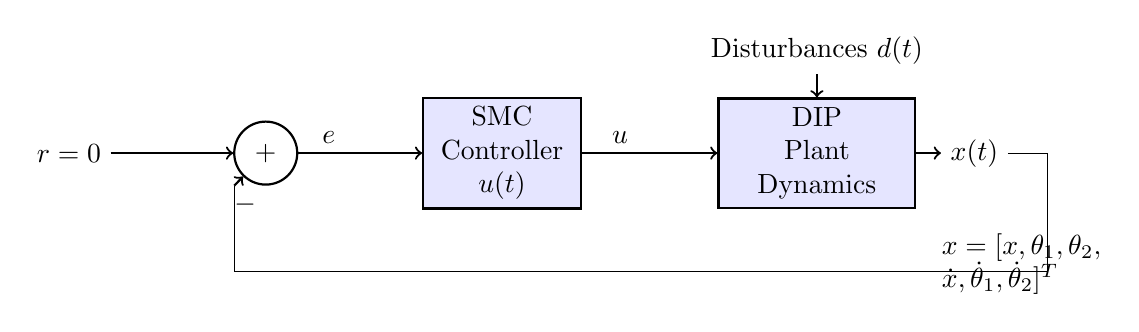
\begin{tikzpicture}[
    block/.style={rectangle, draw, thick, fill=blue!10, minimum height=1cm, minimum width=2cm, align=center},
    sum/.style={circle, draw, thick, minimum size=0.8cm},
    arrow/.style={->, thick},
    node distance=2.5cm
]
    % Reference input
    \node (ref) {$\vect{r} = \vect{0}$};

    % Summing junction
    \node[sum, right of=ref] (sum) {$+$};
    \draw[arrow] (ref) -- (sum);

    % Error signal
    \coordinate[right of=sum, node distance=0.8cm] (err);
    \node[above] at (err) {$\vect{e}$};

    % SMC Controller
    \node[block, right of=sum, node distance=3cm] (controller) {SMC\\Controller\\$u(t)$};
    \draw[arrow] (sum) -- (controller);

    % Control signal
    \coordinate[right of=controller, node distance=1.5cm] (ctrl);
    \node[above] at (ctrl) {$u$};

    % DIP Plant
    \node[block, right of=controller, node distance=4cm, minimum width=2.5cm] (plant) {DIP\\Plant\\Dynamics};
    \draw[arrow] (controller) -- (plant);

    % Output
    \coordinate[right of=plant, node distance=2cm] (output);
    \node[right of=plant, node distance=2cm] (y) {$\vect{x}(t)$};
    \draw[arrow] (plant) -- (y);

    % Feedback path
    \coordinate[below of=plant, node distance=1.5cm] (feedback);
    \draw (y.east) -- ++(0.5, 0) |- (feedback) -| ([xshift=-0.4cm]sum.south);
    \draw[arrow] ([xshift=-0.4cm]sum.south) -- (sum);

    % State labels on feedback
    \node[right, align=left] at ([xshift=0.2cm, yshift=-0.7cm]plant.south east)
        {$\vect{x} = [x, \theta_1, \theta_2,$\\$\dot{x}, \dot{\theta}_1, \dot{\theta}_2]^T$};

    % Disturbances
    \node[above of=plant, node distance=1.3cm] (dist) {Disturbances $d(t)$};
    \draw[arrow] (dist) -- (plant);

    % Negative feedback indicator
    \node[below left] at (sum.south) {$-$};

\end{tikzpicture}

\caption[SMC Control Loop Block Diagram]{Block diagram of the sliding mode control loop architecture. The \textbf{Controller} computes control input $u$ based on state error $\vect{e} = \vect{x}_{\text{ref}} - \vect{x}$ and sliding surface $\sigma$. The \textbf{Plant} (DIP dynamics) evolves according to nonlinear equations of motion. \textbf{Sensors} measure cart position and pendulum angles ($x, \theta_1, \theta_2$) with optional state estimation for velocities. The control law enforces $\dot{\sigma} < 0$ to drive the system toward the sliding manifold $\sigma = 0$, ensuring convergence to equilibrium.}
\label{fig:intro:control_loop}
\end{figure}

\subsection{Key Components}

\subsubsection{Controller Implementations}

All controllers are implemented as Python classes inheriting from a common base:

\begin{itemize}
    \item \pyclass{ClassicalSMC}: First-order SMC with boundary layer
    \item \pyclass{SuperTwistingSMC}: Second-order STA algorithm
    \item \pyclass{AdaptiveSMC}: Online gain adaptation
    \item \pyclass{HybridAdaptiveSTASMC}: Combined adaptive + STA
    \item \pyclass{SwingUpSMC}: Energy-based swing-up with SMC stabilization
\end{itemize}

\subsubsection{Dynamics Models}

Multiple fidelity levels for computational efficiency vs. accuracy trade-offs:

\begin{itemize}
    \item \pyclass{SimplifiedDynamics}: Small-angle approximation, constant inertia matrix (5× faster)
    \item \pyclass{FullDynamics}: Complete nonlinear dynamics with configuration-dependent inertia
    \item \pyclass{LowRankDynamics}: Reduced-order model for Kalman filtering
\end{itemize}

\subsubsection{Optimization Tools}

\begin{itemize}
    \item \pyclass{PSOTuner}: Particle Swarm Optimization for automatic gain tuning
    \item Multi-objective cost functions (tracking error, control effort\index{performance metrics!control effort}\index{performance metrics!control effort}, chattering)
    \item Batch simulation with Numba acceleration (30 particles × 100 iterations in <3 minutes)
\end{itemize}

\subsection{Simulation and Visualization}

\begin{itemize}
    \item \textbf{Command-Line Interface}: \texttt{simulate.py} for quick controller testing
    \item \textbf{Web Interface}: Streamlit\index{Streamlit}\index{Streamlit} app for interactive parameter tuning
    \item \textbf{Real-Time Animation}: DIPAnimator class for phase-space visualization
    \item \textbf{Batch Analysis}: Monte Carlo\index{Monte Carlo simulation} simulations for robustness evaluation
\end{itemize}

\subsection{Getting Started}

\begin{lstlisting}[language=bash, caption={Quick Start Example}, label={lst:intro:quickstart}]
# Clone repository
git clone https://github.com/theSadeQ/dip-smc-pso.git
cd dip-smc-pso

# Install dependencies
pip install -r requirements.txt

# Run classical SMC with default gains
python simulate.py --ctrl classical_smc --plot

# Optimize gains with PSO
python simulate.py --ctrl classical_smc --run-pso --save gains.json

# Load optimized gains and simulate
python simulate.py --ctrl classical_smc --load gains.json --plot
\end{lstlisting}

%%%%%%%%%%%%%%%%%%%%%%%%%%%%%%%%%%%%%%%%%%%%%%%%%%%%%%%%%%%%%%%%%%%%%%%%%%%%%%%%
\section{Book Structure and Learning Path}
\label{sec:intro:structure}

\subsection{Part I: Foundations (Chapters 1--2)}

\begin{itemize}
    \item \textbf{Chapter 1 (Introduction)}: Motivation, history, and overview
    \item \textbf{Chapter 2 (Mathematical Foundations)}: Lagrangian mechanics, Lyapunov stability, controllability theory, numerical integration
\end{itemize}

\subsection{Part II: Controller Design (Chapters 3--7)}

\begin{itemize}
    \item \textbf{Chapter 3 (Classical SMC)}: Sliding surface design, boundary layer theory, Lyapunov proofs
    \item \textbf{Chapter 4 (Super-Twisting)}: Second-order sliding modes, finite-time convergence, implementation
    \item \textbf{Chapter 5 (Adaptive SMC)}: Online gain adaptation, dead zone design, stability analysis
    \item \textbf{Chapter 6 (Hybrid Adaptive STA)}: Combined approach, lambda scheduling, experimental results
    \item \textbf{Chapter 7 (Swing-Up Control)}: Energy-based methods, switching logic, global stability
\end{itemize}

\subsection{Part III: Optimization and Analysis (Chapters 8--10)}

\begin{itemize}
    \item \textbf{Chapter 8 (PSO Optimization)}: Gain tuning, multi-objective cost functions, generalization
    \item \textbf{Chapter 9 (Robustness Analysis)}: Model uncertainty\index{uncertainty}, Monte Carlo simulations, worst-case\index{worst-case analysis} performance
    \item \textbf{Chapter 10 (Benchmarking)}: Performance metrics, statistical analysis, trade-off visualization
\end{itemize}

\subsection{Part IV: Implementation and Advanced Topics (Chapters 11--12)}

\begin{itemize}
    \item \textbf{Chapter 11 (Software Architecture)}: Design patterns, testing strategies, documentation
    \item \textbf{Chapter 12 (Advanced Topics)}: MPC, fractional-order SMC, neural network integration, future directions
\end{itemize}

\subsection{Appendices}

\begin{itemize}
    \item \textbf{Appendix A}: Mathematical prerequisites (linear algebra, ODEs, Lyapunov basics)
    \item \textbf{Appendix B}: Python programming guide for control engineers
    \item \textbf{Appendix C}: Complete controller implementations with annotations
    \item \textbf{Appendix D}: Experimental data tables and benchmark results
    \item \textbf{Appendix E}: Solutions to exercises
\end{itemize}

\subsection{Learning Paths}

\subsubsection{Path 1: Theory-Focused (Graduate Students)}
Chapters 1 $\to$ 2 $\to$ 3 $\to$ 4 $\to$ 5 $\to$ 9 $\to$ 12 (focus on proofs and convergence analysis)

\subsubsection{Path 2: Implementation-Focused (Engineers)}
Chapters 1 $\to$ 3 $\to$ 8 $\to$ 11 $\to$ Appendix C (focus on code and practical tuning)

\subsubsection{Path 3: Research-Focused (PhD Candidates)}
All chapters sequentially + extensive exercises + original experiments

%%%%%%%%%%%%%%%%%%%%%%%%%%%%%%%%%%%%%%%%%%%%%%%%%%%%%%%%%%%%%%%%%%%%%%%%%%%%%%%%
\section{Prerequisites and Notation}
\label{sec:intro:prerequisites}

\subsection{Mathematical Prerequisites}

Readers should be familiar with:

\begin{itemize}
    \item \textbf{Linear Algebra}: Vector spaces, matrices, eigenvalues, definiteness
    \item \textbf{Ordinary Differential Equations}: Existence/uniqueness, stability, Lyapunov theory (basics)
    \item \textbf{Classical Mechanics}: Lagrangian formulation (helpful but not essential)
    \item \textbf{Control Theory}: State-space representation, controllability, feedback linearization\index{linearization} (introductory level)
\end{itemize}

Readers without these prerequisites should consult \cref{app:math_prereq} for a self-contained review.

\subsection{Programming Prerequisites}

The software implementations assume:

\begin{itemize}
    \item Basic Python programming (functions, classes, NumPy\index{NumPy}\index{NumPy} arrays)
    \item Familiarity with scientific computing libraries (NumPy, SciPy\index{SciPy}\index{SciPy}, Matplotlib)
    \item Understanding of object-oriented programming (helpful but not essential)
\end{itemize}

Appendix \ref{app:api} provides an API reference for the Python implementation.

\subsection{Notation Conventions}

\begin{table}[htbp]
\centering
\caption{Notation Guide}
\label{tab:intro:notation}
\begin{tabular}{ll}
\toprule
\textbf{Symbol} & \textbf{Meaning} \\
\midrule
$\vect{x}$ & State vector (bold lowercase) \\
$\mat{M}$ & Matrix (bold uppercase) \\
$\Real^n$ & $n$-dimensional real vector space \\
$\dot{x}$ & Time derivative of $x$ \\
$\ddot{x}$ & Second time derivative of $x$ \\
$\pdiff{f}{x}$ & Partial derivative of $f$ with respect to $x$ \\
$\norm{\vect{x}}$ & Euclidean norm of vector $\vect{x}$ \\
$\sign(x)$ & Sign function: $+1$ if $x > 0$, $-1$ if $x < 0$ \\
$\sat(x)$ & Saturation function (boundary layer approximation) \\
$\sigma$ & Sliding surface value \\
$u$ & Control input \\
$\theta_1, \theta_2$ & Pendulum angles \\
$M, m_1, m_2$ & Cart and pendulum masses \\
$L_1, L_2$ & Pendulum lengths \\
\bottomrule
\end{tabular}
\end{table}

%%%%%%%%%%%%%%%%%%%%%%%%%%%%%%%%%%%%%%%%%%%%%%%%%%%%%%%%%%%%%%%%%%%%%%%%%%%%%%%%
\section{Exercises}
\label{sec:intro:exercises}

\begin{exercise}[Underactuation Degree]
Consider a robotic arm with $n$ revolute joints, each with one actuator. How many independent control inputs does this system have? Is it underactuated, fully actuated, or overactuated? What if two joints share a single actuator via a differential mechanism?
\end{exercise}

\begin{exercise}[DIP Controllability]
The double-inverted pendulum has 3 degrees of freedom and 1 actuator. Calculate the degree of underactuation. If we add a second actuator directly controlling $\theta_1$, would the system become fully actuated?
\end{exercise}

\begin{exercise}[Sliding Surface Design]
For a simple inverted pendulum (1 DOF), propose a sliding surface $\sigma(\theta, \dot{\theta})$ such that $\sigma = 0$ implies $\theta \to 0$ exponentially. What constraints must the sliding surface parameters satisfy?
\end{exercise}

\begin{exercise}[Chattering Frequency Estimation]
A discrete-time controller samples at 1 kHz. If the sliding surface value oscillates with amplitude $\pm 0.01$ and the system derivative $\dot{\sigma} \approx 10$, estimate the chattering frequency. How does doubling the sampling rate affect this?
\end{exercise}

\begin{exercise}[Energy Analysis]
Write the total mechanical energy of the DIP system as $E = T + V$ (kinetic + potential). At the upright equilibrium $(\theta_1 = \theta_2 = 0, \dot{\theta}_1 = \dot{\theta}_2 = 0)$, is this energy a local minimum, maximum, or saddle point?
\end{exercise}

\begin{exercise}[Lyapunov Function Selection]
For the sliding surface $\sigma = k_1 \theta + k_2 \dot{\theta}$ with $k_1, k_2 > 0$, verify that $V = \frac{1}{2} \sigma^2$ is a valid Lyapunov function (positive definite, radially unbounded). Under what conditions is $\dot{V} < 0$?
\end{exercise}

\begin{exercise}[Boundary Layer Trade-off]
If the boundary layer thickness $\epsilon$ is doubled, how does the steady-state tracking error change? How does the chattering frequency change? Derive these relationships analytically assuming a first-order approximation.
\end{exercise}

\begin{exercise}[Historical Context]
Research Vadim Utkin's 1977 paper~\cite{utkin1977variable}. Summarize the three main theoretical contributions and explain how they differ from prior variable structure control work.
\end{exercise}

%%%%%%%%%%%%%%%%%%%%%%%%%%%%%%%%%%%%%%%%%%%%%%%%%%%%%%%%%%%%%%%%%%%%%%%%%%%%%%%%
\section{Chapter Summary}
\label{sec:intro:summary}

This chapter established the foundation for the remainder of the book:

\begin{itemize}
    \item \textbf{Underactuation} is a fundamental challenge in robotics and control, arising when the number of actuators is less than the number of degrees of freedom
    \item The \textbf{double-inverted pendulum} serves as an ideal benchmark: challenging dynamics, well-defined control objectives, and hardware realizability
    \item \textbf{Sliding Mode Control} has evolved from 1950s variable structure systems to modern adaptive and higher-order algorithms
    \item The \textbf{chattering problem} remains the primary practical limitation, addressed through boundary layers, higher-order sliding modes, and adaptive methods
    \item This book presents \textbf{five controllers} (Classical SMC, STA, Adaptive, Hybrid, Swing-Up), rigorously derived and implemented in production-quality Python
    \item The accompanying \textbf{software framework} provides modular, tested, and optimized implementations suitable for research and deployment
\end{itemize}

\textbf{Next Steps}: \cref{ch:mathematical_foundations} develops the mathematical prerequisites for controller design, including Lagrangian mechanics, Lyapunov stability theory, and numerical integration methods. Readers already familiar with these topics may proceed directly to \cref{ch:classical_smc}.

%%%%%%%%%%%%%%%%%%%%%%%%%%%%%%%%%%%%%%%%%%%%%%%%%%%%%%%%%%%%%%%%%%%%%%%%%%%%%%%%
% End of Chapter 1
%%%%%%%%%%%%%%%%%%%%%%%%%%%%%%%%%%%%%%%%%%%%%%%%%%%%%%%%%%%%%%%%%%%%%%%%%%%%%%%%
